\scanpage{20}
\figure{
\begin{tikzpicture}
\node[draw,circle,inner sep=3pt] {\mspage{7}};
\end{tikzpicture}}

\diagram{\begin{tikzcd}[ampersand replacement=\&,column sep=1.6em,row sep=2.8em]
\&\&
\begin{gathered}
\widetilde\rho=(\rho_0,2)=(\rho,2)\\
\widetilde\sigma=(\sigma_0,3)=(\sigma,3)
\end{gathered}
\arrow[d, bend right=20]
\&
\begin{gathered}
\deleted{\unsure{\Pi_{0,3}^{D}}}\\[-2pt]
\inserted{\text{\uline{\unsure{identified with}}}}\\[-2pt]
\inserted{\unsure{S\mathcal T_{11}\times_{\Pi_{0,3}^{D}}\mathbb Z/12\mathbb Z}}
\end{gathered}
\arrow[d]
\&
\begin{gathered}
\rho_0=(\rho,\dot 2)\\[-2pt]
\unsure{\Pi_{0,3}}\\[-2pt]
\sigma_0=(\sigma,\dot 3)=(\sigma,-1)
\end{gathered}
\arrow[d]
\&\\
\unsure{0|1}\arrow[r,dash]\&
\mathbb Z\arrow[r,dash,"1\unsure{-|\mapsto}\overline\omega=\omega^2"]\arrow[dd,equal]\&
S\mathcal T_{11}\arrow[r,Rightarrow]\arrow[dd,"\substack{\widetilde\rho\mapsto\deleted{\unsure{4}}2\\\widetilde\sigma\mapsto3}"']
\arrow[ddr,phantom,"\text{Cartesian}"]\&
\mathcal T_{11}\arrow[r,Rightarrow]\arrow[dr,leftrightarrow]\arrow[dd,"\substack{\rho_0\mapsto\dot 2\\\sigma_0\mapsto\dot 3}"']
\&\Pi_{0,3}^{\prime D}\arrow[dr,"\text{canonical}"]\arrow[dd,"\substack{\rho\mapsto2\\\sigma\mapsto3}"{pos=.25,xshift=2pt}]
\arrow[dl,phantom,"\text{cartesian}" description]\&\\
\&\&\&{}\&
|[xshift=-3em]|\mathbb D'_3\arrow[r,"\text{cartesian}"{pos=.75}]\arrow[dd]
\&\mathbb D_3\arrow[dd,"\text{canonical}"]\\
1\arrow[r,dash]\&\mathbb Z\arrow[r,"12"]\&\mathbb Z\arrow[r,"\text{canonical}"]\&
\mathbb Z/12\mathbb Z\arrow[r,"\text{canonical}"]\arrow[dr,"\text{canonical}"']
\&\mathbb Z/6\mathbb Z\arrow[dr,"\text{canonical}"]
\arrow[d,phantom,"\text{\uline{Cartesian}}"'{pos=.25,xshift=-3em}]
\arrow[dr,phantom,"\text{\uline{cartesian}}"{description,xshift=-1.5em,yshift=.5em}]\&\\
\&\&\&\&\mathbb Z/4\mathbb Z\arrow[r,leftrightarrow,"\text{canonical}"]\&\mathbb Z/2\mathbb Z
\end{tikzcd}}

\margin{\unsure{for} $\mathcal T_{11}$ \unsure{identified with}
$\Pi_{0,3}^{D}\times_{\mathbb Z/2\mathbb Z}\mathbb Z/4\mathbb Z$}

\unsure{Have we} \unsure{indeed}\quad
$\bigm|\quad S\mathcal T_{11}\simeq S\Pi_{0,3}^{D}$ ??

it would rather seem, however
\[
\deleted{\unsure{\mathcal T_{11}}}\quad
PM_{11}\simeq
\left(\underbrace{T^*U_{0,3}}_{\substack{\text{bundle}\\\text{\uline{tangent}}}},\mathfrak S_3\right)
\]
\inserted{(and \uline{not} $\unsure{PU_{0,3}}$ !!)}

\[
\text{thus}\quad \mathcal T_{11}\simeq\pi_1(T^*U_{0,3},\mathfrak S_3)\ \ldots
\]
\margin{19}

\scanpage{21}
% Trois longs traits obliques au crayon, terminés chacun en crochet, traversent tout le feuillet : rature d'ensemble.
% Les ratures à l'encre (ligne « Op. ext. … », « compatible avec l'op. ext. », E corrigé en F, 1 et π_1 de la dernière suite) restent marquées à l'intérieur.
\deleted{
\[
\pi\qquad l_1\ \cdots\ l_n
\]

\diagram{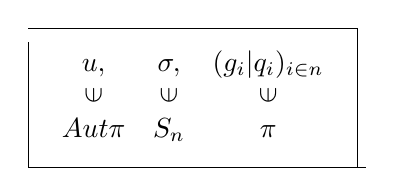
\begin{tikzpicture}
\node[inner sep=7pt] (p) {$\begin{array}{ccc}
u,&\sigma,&(\unsure{g_i|q_i})_{i\in n}\\
\rotatebox{90}{$\in$}&\rotatebox{90}{$\in$}&\rotatebox{90}{$\in$}\\
\operatorname{Aut}\pi&\mathfrak S_n&\pi
\end{array}$};
\draw (p.north west) -- (p.north east) -- (p.south east);
\draw ([yshift=-5pt]p.north west) -- (p.south west) -- ([xshift=3pt]p.south east);
\end{tikzpicture}}
\diagram{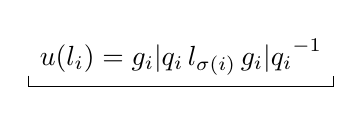
\begin{tikzpicture}
\node[inner sep=4pt] (u) {$u(l_i)=\unsure{g_i|q_i}\,l_{\sigma(i)}\,\unsure{g_i|q_i}^{-1}$};
\draw ([yshift=4pt]u.south west) -- (u.south west) -- (u.south east) -- ([yshift=4pt]u.south east);
\end{tikzpicture}}

\diagram{\begin{tikzcd}[ampersand replacement=\&,column sep=1.5em]
1\arrow[r,dash]\&\pi_1(\operatorname{Aut}(X)\arrow[r]\&\mathbb Z^n\arrow[r]\&S\mathcal T\arrow[r]\&\mathcal T\arrow[r,dash]\&\mathfrak S_n\arrow[r,dash]\&1
\end{tikzcd}}

\diagram{\begin{tikzpicture}
\node[inner sep=9pt] (b) {\begin{tikzcd}[ampersand replacement=\&,column sep=3em,row sep=2.5em]
\pi\arrow[r,hook]\&\widetilde E\arrow[r]\arrow[d,leftrightarrow]\&\mathfrak S_n\\
\unsure{\mathfrak Z\pi|\mathfrak z\pi}\arrow[u]\arrow[r]\&\mathbb Z^n\&{}
\end{tikzcd}};
\draw (b.north west) -- (b.north east) -- ([yshift=2pt]b.east) -- ([xshift=-6pt]b.east)
 -- ([xshift=-12pt,yshift=5pt]b.south east) -- ([xshift=0.7cm,yshift=5pt]b.south)
 -- ([xshift=0.6cm,yshift=-6pt]b.south) -- ([yshift=-6pt]b.south west) -- (b.north west);
\end{tikzpicture}}

\diagram{\begin{tikzcd}[ampersand replacement=\&,column sep=2.3em,row sep=1.8em]
\&\&1\&\&\\
1\arrow[r]\&\underbrace{S\operatorname{Aut}^{+}(X)}\arrow[r]\arrow[d,"\simeq"]\&
\operatorname{Aut}^{+}(X)\arrow[u]\arrow[r,dash]\&\operatorname{Aut}^{+}(\partial X)\arrow[r,dash]\&1\\
\&\uline{S\mathcal T}\&\operatorname{Aut}^{+}_{!}(\widetilde X)\arrow[u]\&\uline{\mathfrak S_n\cdot\mathbb T^n}\arrow[u,"\simeq"]\&\\
\&\&\pi\arrow[u]\&\&\\
\&\&1\arrow[u]\&\&
\end{tikzcd}}

\diagram{\begin{tikzcd}[ampersand replacement=\&,column sep=1.6em]
1\arrow[r,dash]\&\underbrace{\pi_1\operatorname{Aut}^{+}(X)}_{0\ \text{or}\ \mathbb Z}\arrow[r,Rightarrow]\&\mathbb Z^n\arrow[r,dash]\&S\mathcal T\arrow[r,dash]\&\mathcal T\arrow[r,dash]\&\mathfrak S_n\arrow[r,dash]\&1
\end{tikzcd}}

\diagram{\begin{tikzpicture}
\node[inner sep=6pt] (e) {\begin{tikzcd}[ampersand replacement=\&,column sep=2em,row sep=1.8em]
1\arrow[r,dash]\&S\mathcal T\arrow[r,dash]\&E\arrow[r]\arrow[d,equal]\&\mathfrak S_n\arrow[r,dash]\&1\\
\&\mathbb Z^n\arrow[u]\&\widetilde E/\pi\&\&{}
\end{tikzcd}};
\draw ([xshift=5pt]e.north west) -- ([xshift=-7pt]e.north east)
 .. controls ([xshift=12pt]e.north east) and ([xshift=12pt,yshift=-1cm]e.north east) .. ([xshift=-4pt,yshift=-1.1cm]e.north east)
 -- ([xshift=-0.5cm,yshift=-1.1cm]e.north)
 .. controls ([xshift=-0.8cm,yshift=-1.2cm]e.north) and ([xshift=-0.8cm,yshift=-0.3cm]e.south) .. ([xshift=-1.5cm]e.south)
 .. controls (e.south west) and ([xshift=-8pt]e.west) .. ([yshift=-4pt]e.north west);
\end{tikzpicture}}

\diagram{\begin{tikzcd}[ampersand replacement=\&,column sep=2.4em,row sep=2em]
1\arrow[r,dash]\&\unsure{\widetilde F|\widehat F}\arrow[r,dash]\arrow[d]\&\widetilde A\arrow[r,dash]\arrow[d]\&\widetilde G\arrow[d]\&\\
1\arrow[r,dash]\&\substack{\deleted{\unsure{E}}\inserted{F}\\\text{discrete}}\arrow[r]\&A\arrow[r]\&G\arrow[dr]\&
\bigl(=\mathfrak S_n\unsure{\ast|\cdot}\mathbb T^n\bigr)\\
\&\&\&\&1
\end{tikzcd}}

\deleted{\unsure{Operation} by outer automorphisms of $\pi_0$ on $F$}

\diagram{\begin{tikzcd}[ampersand replacement=\&,column sep=3.8em,row sep=2.3em]
\pi_1(G)=\pi_1\arrow[r]\arrow[dr,bend right=20,"\substack{\text{\unsure{compatible}}\\\text{with }\pi_0}"']\&F\arrow[d,phantom,"\cup" description]\\
\&\unsure{\mathfrak Z(F)|\mathfrak z(F)}
\end{tikzcd}}
\inserted{\unsure{central}}

$\pi_0(G)=\pi_0$ operates \unsure{by outer automorphisms} on $F$
\quad hence operates on $\unsure{\mathfrak Z(F)|\mathfrak z(F)}$

\diagram{$\begin{array}{cc}
\pi_0&\pi_1\\
\multicolumn{2}{c}{\text{operation}}
\end{array}$}
\deleted{\unsure{compatible} with the outer operation}

\diagram{\begin{tikzcd}[ampersand replacement=\&,column sep=2.4em,row sep=1.7em]
1\arrow[r,dash]\&F\arrow[r]\&E\arrow[r]\arrow[d,equal]\&\pi_0\arrow[r,dash]\&1\\
\&\&\pi_0(\widetilde A)\&\&{}
\end{tikzcd}}
\figure{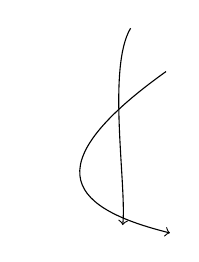
\begin{tikzpicture}[x=1cm,y=1cm]
\draw[->] (0.3,2.5) .. controls (0.0,2.0) and (0.25,0.5) .. (0.2,0);
\draw[->] (0.75,1.95) .. controls (-1.0,0.7) and (-0.4,0.2) .. (0.8,-0.1);
\end{tikzpicture}}

\diagram{\begin{tikzcd}[ampersand replacement=\&,column sep=1.6em]
1\arrow[r,dash]\&\pi_1(A)\arrow[r,dash]\&\pi_1\arrow[r]\&\unsure{F}\arrow[r]\&\underbrace{\pi_0(A)}\arrow[r]\&\substack{\unsure{\pi_0|\pi_\infty}\\ /}\arrow[r,dash]\&1
\end{tikzcd}}

\diagram{\begin{tikzcd}[ampersand replacement=\&,column sep=1.7em,row sep=1.5em]
\deleted{\unsure{1}}\arrow[r,dash]\&\deleted{\unsure{\pi_1}}\arrow[r,dash]\&F\arrow[r,dash]\&\pi_0(\widetilde A)\arrow[r]\arrow[d,equal]\&\pi_0\arrow[r]\&1\\
\&\&\&E\&\&{}
\end{tikzcd}}
}
\margin{20}

\scanpage{22}
% blank
\margin{21}

\scanpage{23}
A)\quad \uline{Lemma}\quad
$S$ \deleted{\unsure{satisfying|strictly}}
regular integral scheme such that $\operatorname{Pic}(S)=0$,
characteristic of the generic point $\ne2$ Then \deleted{$\unsure{H^1}$}
\[
H^1(U_{0,3},\mathfrak S_3;\mathbb G_m]\simeq\mathbb Z/6\mathbb Z
\]
(\deleted{\unsure{residual}}\inserted{\unsure{generic point|if generic}} is $2$, we find $\mathbb Z/3\mathbb Z$)

\margin{\uline{\unsure{Proof}}\quad we use exact sequence
\diagram{\begin{tikzcd}[ampersand replacement=\&,column sep=1.3em,row sep=2em]
0\arrow[r]\&H^1(\mathfrak S_3,H^0(U_{0,3},\mathbb G_m)\arrow[r]\&H^1(\text{mixed})\arrow[dll]\&{}\\
H^0\bigl(\mathfrak S_3,\underbrace{H^1(U_{0,3};\mathbb G_m)}_{0}\bigr)\&\&\&{}
\end{tikzcd}}
and
\diagram{\begin{tikzcd}[ampersand replacement=\&,column sep=1.3em]
0\arrow[r]\&H^0(S,\mathbb G_m)\arrow[r]\&H^0(U_{0,3},\mathbb G_m)\arrow[r]\&\unsure{h_1(V(J))|h^1(V(J))}\arrow[r]\&0
\end{tikzcd}}}

\unsure{I} say that if \inserted{the scheme}
$\deleted{\unsure{U_{0,3}}}\inserted{\Sigma_J}$ is defined as $\mathbb P(V_J)$, \unsure{i.e.}
\diagram{\begin{tikzcd}[ampersand replacement=\&,column sep=2.8em]
0\arrow[r,dash]\&V_J\arrow[r]\&\mathcal O^J\arrow[r]\&\mathcal O\arrow[r,dash]\&0
\end{tikzcd}}
then the \unsure{principal} bundle
\[
P\Sigma_J=\check V(\mathcal O_{\Sigma_J}(1))^{*}
\]
is a generator of the
$H^1(\deleted{\unsure{U_{0,3}}}\inserted{\Sigma_J^*},
\deleted{\unsure{\mathfrak S_3}}\inserted{\mathfrak S_J};\mathbb G_m)$.

I will first \unsure{find} a trivialization of
\[
\uline{\mathcal O}(1)^{\otimes6}=\mathcal O(6)\simeq
\unsure{\mathcal T^{\otimes3}(\omega)|\mathcal J^{\otimes3}(\omega)},
\]
\deleted{thus} \inserted{in fact} a section of $\mathcal O(6)$
\inserted{over $\overline\Sigma$ \unsure{in its entirety}}
(which \deleted{\unsure{vanishes only}}
\inserted{\unsure{is}, \unsure{invertible}} on $\Sigma^*$.
We \deleted{\unsure{taking}} have
\[
\Gamma(\Sigma_J,\mathcal O(6))\simeq\operatorname{Sym}^{6}V_J
\]
and we will take
\[
\begin{gathered}
\unsure{\varphi|\Delta}\in\Gamma(\Sigma_J,\mathcal O(6)),\qquad
\unsure{\varphi|\Delta}
=\deleted{\unsure{\sum_{i\in J}}}
-\prod_{\substack{i,j\in J\\i\ne j}}(e_i-e_j)\\
=\prod_{i\in J}\underbrace{(e_j-e_h)}_{J=\{i,j,h\}}^{2}.
\end{gathered}
\]
Thus, over $\deleted{\unsure{U_J}}\inserted{\Sigma_J^{*}}$, the \unsure{structure|structure} group
\deleted{\unsure{of}}
$\mathbb G_m$ of $P\Sigma_J^{*}$ is reduced \unsure{to|:} $\mu_6$.

\uline{N.B.}\quad Unless I am mistaken, we have
\[
\deleted{\unsure{\operatorname{Sym}}}\quad
\operatorname{Sym}^{*}(V_J)^{\mathfrak S_3}\simeq
\mathcal O\bigl(\unsure{\gamma_2|\varphi_2},\unsure{\gamma_3|\varphi_3}\bigr)
/(2\gamma_3^2-\gamma_2^3)
\]
\[
\left\{\begin{aligned}
\gamma_2&=\sum_{i\in J}(e_j-e_h)^2\\
\gamma_3&=\prod_{i\in J}(e_j\unsure{-|+}e_h-2e_i)
\end{aligned}\right.
\qquad\text{and}\quad\Delta=\gamma_2^3
\]
\margin{22}

\scanpage{24}
% not manuscript: tract imprimé « Parler Femmes à propos de “PLURIELLES” », avec une longue rature diagonale.
\margin{23}

\scanpage{25}
B)

\deleted{\unsure{If} $2$ \unsure{invertible}, we \unsure{will have} \unsure{therefore}}
\[
\deleted{\operatorname{Sym}^{*}(\unsure{V_J|W_J})^{\mathfrak S_{\unsure{J|3}}}\simeq\mathcal O[}
\]
\deleted{\unsure{Remark}}

Since $\gamma_2$ vanishes at \deleted{\unsure{the}} $P_\omega$,
$\gamma_3$ at the $Q_i$, it follows that there is no invariant section
of an $\mathcal O(n)^*$ \deleted{\unsure{for}} over
$\Sigma_J^{*}$ \deleted{\unsure{in degree} $<$}
for $n\le6$, hence that the order of
$\operatorname{cl}(\mathcal O(1))$ in
$H^1(\Sigma_J,\mathfrak S_J;\mathbb G_m)$ is indeed $6$,
which \unsure{proves} that $\mathcal O(1)$ is a generator of the
mixed $\unsure{H^1}$.
\margin{24}
\scanpage{26}
% not manuscript: feuillet dactylographié « Sciences de l’homme », « Energie », « Mécanique et industries de transformation », « Recherches sur les milieux tropicaux et sub-tropicaux » ; pagination imprimée « - 4 - ».
\margin{25}